%%%%%%%%%%%%%%%%%%%%%%%%%%%%%%%%%%%%%%%%%%%%%%%%%%%%%%%%%%%%%%
%%%%%%%%%%%%%%%%%%%%%%%%%%%%%%%%%%%%%%%%%%%%%%%%%%%%%%%%%%%%%%
%%                                                          %%
%% Important note on usage                                  %%
%% -----------------------                                  %%
%% This file should normally be compiled with PDFLaTeX      %%
%% Using standard LaTeX should work but may produce clashes %%
%%                                                          %%
%%%%%%%%%%%%%%%%%%%%%%%%%%%%%%%%%%%%%%%%%%%%%%%%%%%%%%%%%%%%%%
%%%%%%%%%%%%%%%%%%%%%%%%%%%%%%%%%%%%%%%%%%%%%%%%%%%%%%%%%%%%%%%

%% The '3p' and 'times' class options of elsarticle are used for Elsevier CRC
%% Add the 'procedia' option to approximate to the Word template
%\documentclass[3p,times,procedia]{elsarticle}
\documentclass[3p,times]{elsarticle}

%% The `ecrc' package must be called to make the CRC functionality available
\usepackage{ecrc}

%% The ecrc package defines commands needed for running heads and logos.
%% For running heads, you can set the journal name, the volume, the starting page and the authors

%% set the volume if you know. Otherwise `00'
\volume{00}

%% set the starting page if not 1
\firstpage{1}

%% Give the name of the journal
\journalname{Future Generation Computing Systems}

%% Give the author list to appear in the running head
%% Example \runauth{C.V. Radhakrishnan et al.}
\runauth{L. Miroslaw et al.}

%% The choice of journal logo is determined by the \jid and \jnltitlelogo commands.
%% A user-supplied logo with the name <\jid>logo.pdf will be inserted if present.
%% e.g. if \jid{yspmi} the system will look for a file yspmilogo.pdf
%% Otherwise the content of \jnltitlelogo will be set between horizontal lines as a default logo

%% Give the abbreviation of the Journal.  Contact the journal editorial office if in any doubt
\jid{fgcs}

%% Give a short journal name for the dummy logo (if needed)
\jnltitlelogo{FGCS}

%% Provide the copyright line to appear in the abstract
%% Usage:
%   \CopyrightLine[<text-before-year>]{<year>}{<restt-of-the-copyright-text>}
%   \CopyrightLine[Crown copyright]{2011}{Published by Elsevier Ltd.}
%   \CopyrightLine{2011}{Elsevier Ltd. All rights reserved}
\CopyrightLine{2011}{Published by Elsevier Ltd.}

%% Hereafter the template follows `elsarticle'.
%% For more details see the existing template files elsarticle-template-harv.tex and elsarticle-template-num.tex.

%% Elsevier CRC generally uses a numbered reference style
%% For this, the conventions of elsarticle-template-num.tex should be followed (included below)
%% If using BibTeX, use the style file elsarticle-num.bst

%% End of ecrc-specific commands
%%%%%%%%%%%%%%%%%%%%%%%%%%%%%%%%%%%%%%%%%%%%%%%%%%%%%%%%%%%%%%%%%%%%%%%%%%

%% The amssymb package provides various useful mathematical symbols
\usepackage{amssymb}
\usepackage{url}
%% The amsthm package provides extended theorem environments
%% \usepackage{amsthm}

%% The lineno packages adds line numbers. Start line numbering with
%% \begin{linenumbers}, end it with \end{linenumbers}. Or switch it on
%% for the whole article with \linenumbers after \end{frontmatter}.
%\usepackage{lineno}

%% natbib.sty is loaded by default. However, natbib options can be
%% provided with \biboptions{...} command. Following options are
%% valid:

%%   round  -  round parentheses are used (default)
%%   square -  square brackets are used   [option]
%%   curly  -  curly braces are used      {option}
%%   angle  -  angle brackets are used    <option>
%%   semicolon  -  multiple citations separated by semi-colon
%%   colon  - same as semicolon, an earlier confusion
%%   comma  -  separated by comma
%%   numbers-  selects numerical citations
%%   super  -  numerical citations as superscripts
%%   sort   -  sorts multiple citations according to order in ref. list
%%   sort&compress   -  like sort, but also compresses numerical citations
%%   compress - compresses without sorting
%%
%% \biboptions{comma,round}

% \biboptions{}

% if you have landscape tables
\usepackage[figuresright]{rotating}

% put your own definitions here:
%   \newcommand{\cZ}{\cal{Z}}
%   \newtheorem{def}{Definition}[section]
%   ...

% add words to TeX's hyphenation exception list
%\hyphenation{author another created financial paper re-commend-ed Post-Script}

% declarations for front matter

\usepackage[utf8]{inputenc} % set input encoding (not needed with XeLaTeX)
\usepackage{wrapfig} 
\usepackage{subcaption}
\usepackage{graphicx} % support the \includegraphics command and options

%%% PACKAGES
%\usepackage{booktabs} % for much better looking tables
%\usepackage{tikz}
\usepackage{todonotes}
%\usepackage{array} % for better arrays (eg matrices) in maths
%\usepackage{paralist} % very flexible & customisable lists (eg. enumerate/itemize, etc.)
%\usepackage{verbatim} % adds environment for commenting out blocks of text & for better verbatim
%\usepackage{subfig} % fmake it possible to include more than one captioned figure/table in a single float
% These packages are all incorporated in the memoir class to one degree or another...

%%% SECTION TITLE APPEARANCE
%\usepackage{sectsty}
%\allsectionsfont{\sffamily\mdseries\upshape} % (See the fntguide.pdf for font help)
% (This matches ConTeXt defaults)

%%% ToC (table of contents) APPEARANCE
%\usepackage[nottoc,notlof,notlot]{tocbibind} % Put the bibliography in the ToC
%\usepackage[titles,subfigure]{tocloft} % Alter the style of the Table of Contents
%\renewcommand{\cftsecfont}{\rmfamily\mdseries\upshape}
%\renewcommand{\cftsecpagefont}{\rmfamily\mdseries\upshape} % No bold!

%%% END Article customizations

\DeclareGraphicsExtensions{.pdf,.png,.jpg}
\graphicspath{ {../figs/} }

\begin{document}

\begin{frontmatter}

%% Title, authors and addresses

%% use the tnoteref command within \title for footnotes;
%% use the tnotetext command for the associated footnote;
%% use the fnref command within \author or \address for footnotes;
%% use the fntext command for the associated footnote;
%% use the corref command within \author for corresponding author footnotes;
%% use the cortext command for the associated footnote;
%% use the ead command for the email address,
%% and the form \ead[url] for the home page:
%%
%% \title{Title\tnoteref{label1}}
%% \tnotetext[label1]{}
%% \author{Name\corref{cor1}\fnref{label2}}
%% \ead{email address}
%% \ead[url]{home page}
%% \fntext[label2]{}
%% \cortext[cor1]{}
%% \address{Address\fnref{label3}}
%% \fntext[label3]{}

\dochead{Big Data in the Cloud}
%% Use \dochead if there is an article header, e.g. \dochead{Short communication}
%% \dochead can also be used to include a conference title, if directed by the editors
%% e.g. \dochead{17th International Conference on Dynamical Processes in Excited States of Solids}

\title{Unified cloud orchestration framework for elastic high performance computing in the cloud}


%% use optional labels to link authors explicitly to addresses:
%% \author[label1,label2]{<author name>}
%% \address[label1]{<address>}
%% \address[label2]{<address>}

\author[hsr,pwr]{Lukasz Miroslaw}
\author[hsr]{Michael Pantic}
%\author[hsr]{Vladimir Baros}
\author[hsr]{Henrik Nordborg}

\address[hsr]{Institute for Energy Technology, Hochschule Rapperswil, Switzerland}
%\address[eth]{ETH Zurich, Switzerland}
\address[pwr]{Wroclaw University of Technology, Poland}

\begin{abstract}
The demand for computational power and storage in industry and academia is continuously increasing. One of the key drivers of this demand is the increased use of numerical simulations, such as Computational Fluid Dynamics (CFD) for product development. This type of simulations generates huge amounts of data and demands massively parallel computing power. Traditionally, this computational power is provided by large on-premises clusters, which require large investments in hardware and maintenance. The large costs, the lack of flexibility and a high complexity prevent small and medium sized companies from implementing such clusters. Cloud computing has become a viable alternative, offering more flexibility at significantly lower costs but the deployment of numerical applications is time-consuming, error-prone and requires a high level of expertise. The purpose of this paper is to demonstrate the SimplyHPC framework that automatizes the deployment of the cluster in the cloud, deploys and executes large scale and parallel numerical simulations, and finally downloads the results and shuts down the cluster. Using this tool, we have been able to successfully run the widely accepted solvers, namely PETSc, HPCG and ANSYS CFX, in a performant and scalable manner on Microsoft Azure. It has been shown that the cloud computing performance is comparable to on-premises clusters in terms of efficiency and scalability and should be considered as an economically viable alternative. 



\end{abstract}

\begin{keyword}
Microsoft azure \sep high performance computing
%% keywords here, in the form: keyword \sep keyword

%% PACS codes here, in the form: \PACS code \sep code

\MSC[2010] 74F10 \sep 68Uxx	\sep 65Y20
%% MSC codes here, in the form: \MSC code \sep code
%% or \MSC[2008] code \sep code (2000 is the default)

\end{keyword}

\end{frontmatter}

%\linenumbers 

\section{Introduction} 
\label{sec:introduction}

Numerical simulations have become an essential part of modern R\&D, as they allow companies to develop smarter products faster. Ideally, computer simulations can be used to test the performance of a product before the first prototype has been built, providing valuable information very early in the product development cycle. Computer simulations also allow companies to test a large number of design variation and to use numerical optimization algorithms to improve the performance of products.
 
Computational fluid dynamics (or CFD for short) represents the greatest challenge in terms of computational requirements. This kind of simulations can only be used efficiently on parallel compute clusters with hundreds of CPU cores connected through a fast high-performance network such as Infiniband. Unfortunately, such a computational infrastructure represents a significant investment and only makes sense if the computational cluster is heavily utilized to amortize the costs. This is generally not an issue for universities and research institutes, but represents a real problem for profit driven companies, who only occasionally need access to significant computing power. An underutilized compute cluster is simply too expensive to maintain.
 
Most modern CFD solvers support parallel processing through the Message Passing Interface\cite{MPI}. Recently, support for multi-core processors, GPUs, and the Intel Phi have begun to be implemented \cite{tomczak2013} \cite{Che09042015}. Generally speaking, CFD simulation are very well suited for parallel processing. They can be easily parallelized using domain decomposition and the computational performance is mainly limited by memory bandwidth. In addition, the linear equations are reasonably well conditioned and therefore suitable for scalable linear solvers. Finally, the simulations typically produce enormous amounts of data, making the Big Data an issue for computer aided engineering (CAE).

A commonly used CFD tool in industry and research is CFX by ANSYS Inc. The company is one of the largest player in the Computer Aided Engineering (CAE) market \cite{mcae2012} and its software is typically used for the largest simulations composed of millions of cells. Big Data in the CAE domain has become a challenge for HPC engineers as it requires larger and larger clusters and only recently, a shift towards cloud-based solution has been observed.

Cloud computing has become ubiquitous due to its flexibility and cost-efficiency. It has clear advantages over traditional on-premise systems for institutions with limited budgets as no direct investments are needed and machines can be rented on an hourly basis. Users benefit from the cloud through the possibility of launching jobs of different sizes on dynamically sized systems and the cloud operators achieve economies of scale by building large data centers where the resources can be shared between different workloads. \\
An increasing amount of computing power is now hosted on cloud platforms such as Amazon Elastic Compute (EC2) \cite{ec2}, Cloud Foundry Google Compute Engine \cite{google} or Microsoft Azure \cite{azure} and more and more software and services are being hosted in the cloud. Many independent software vendors (ISV) started to offer cloud services to scale scientific applications for specific industries. Many ISVs like Rescale, Ciespace, Ubercloud, Sabalcore, Univa, Penguin Computing provide cloud services for weather research, computational fluid dynamics, structural mechanics, quantitative finance, combustion, electromagnetics and molecular dynamics \cite{theuebercloud}. They offer access to VMs with pre-installed software or a web portal where the scientific applications, such as ANSYS, Gromacs, OpenFOAM or Gerris solvers can be executed \cite{Popinet2003}.

While this may be a satisfying solution for some, the ability to run custom or third-party software on the cloud infrastructure requires much more complicated procedures. A scientific application that needs to be deployed in the Cloud usually consists of a command line-tool that requires complex deployment steps such as installation, configuration as well as setting up system specific services and network policies, comparable to the effort of administering a on-premises cluster. Access to the deployed applications from a local machine is also a tedious procedure and requires a significant amount of effort. This partly explains why this scenario is often too cumbersome for a domain engineer or a scientist.  

A simple mechanism is needed to simplify the whole process and lower the entry barrier for cloud-based numerical simulations. Such mechanisms exist for Amazon EC2 \cite{ec2} \cite{eucalyptus} but Microsoft Azure still lacks an easy-to-use framework to simplify cloud  orchestration, although it is a platform that is well positioned on the market \cite{Garg2013}.

We present a unified framework, named ''SimplyHPC'',  that greatly simplifies the use of a distributed application on Microsoft Azure. The framework combines Azure specific HPC libraries, deployment tools, machine and MPI configuration into a common platform. Its functionality is, among others, exposed through PowerShell commandlets that ease the submission process while keeping the desired command line environment and flexibility. The framework provides tools with the ability to deploy an arbitrary number of virtual machines dynamically, submit the packed application together with input and configuration files, execute it as a cloud service using Message Passing Interface (MPI) and, once the results are ready, download them to the local machine and stop the virtual machines. 

Our paper focuses on the following aspects. Chapter \ref{sec:architecture} describes the main components of the proposed framework as well as the platform architecture. Chapter \ref{sec:results} demonstrates the utility of the tool on two scientific applications, namely PETSc and HPCG. In addition we present the scalability study of ANSYS CFX, a commercial fluid dynamics code for realistic, industrial simulations in a Big Data scenario. The paper ends with conclusions and future plans.

%VERY INTERESTING

%	\item[II] We measured how well different applications scale on a cloud computing platform (Microsoft Azure), evaluating feasibility and %cost of operation for different applications and optimizing the machine count / machine size ratio to get as much GFLOPs per \$ as possible.

%\end{itemize}

\section{Background}
\label{sec:background}
\subsection{Motivation}
Each of the previously mentioned cloud platforms offers different strategies to communicate with the cloud infrastructure and different virtualization procedures. The user is free to manage the cloud resources by deploying the cluster manually or with the help of accompanying scripts and APIs, or use the cloud orchestrators that automate the management of the cloud-based infrastructure. The motivation for our development was twofold.

\begin{description}
\item[Complex deployment] In order to run applications on a cloud, a deployment (installation) of the software is necessary first. In the Infrastructure as a Service (IaaS) approach, the user can access the cloud computers using regular remote desktop infrastructure and therefore manual/scripted installation for each node has to be done (similar to on-premises clusters). In the Platform as a Service (Paas) approach, usually accesses the cloud computers using pre-defined high-level interfaces and therefore has to use pre-installed software or submit his desired application as pre-packaged templates, which need expertise to create. For both approaches, so called \textit{Cloud orchestrators} manage the interactions and interconnections among cloud-based and on-premises business units as well as expose various automated processes and associated resources. They have become a desired alternative to standard deployment procedures because of lower level of expertise and reduced deployment time. Tools for cloud orchestration and vertical and horizontal scaling are fundamental to the adoption of the framework aiming at simplifying the whole procedure.

\item[Complicated access] Although cloud orchestrators play an important role, still there are only a few easy to use, out-of-the box platforms that simplify deployment, monitoring and accessing scientific applications in the cloud. Companies offering cloud-based software in PaaS model limit their offering to applications of the highest commercial impact while neglecting other types of software such as numerical simulations \cite{CloudStack} \cite{OpenStack}. The best situation is in Amazon EC2 where frameworks to simplify the process of orchestration of specific scientific applications exist. Wong and Goscinski propose a unified framework composed of a series of scripts for running gene sequencing analysis jobs through a web portal \cite{Wong2013} on Amazon EC2 (IaaS) infrastructure. For this purpose they designed a HPC service software library for accessing high level HPC resources from the IaaS cloud and demonstrate their framework in running mpiBLAS \cite{mpiBlas}. Balgacem et al. measured the multiphase flow on a hybrid platform combined with Amazon $EC2$ and a private cluster \cite{BenBelgacem2015}. Morpho is a modified version of Hadoop MapReduce framework that decouples storage and computation into physical and virtual clusters to reduce costly data movement of user data \cite{Lu2014}. The authors demonstrate the efficiency of the  framework in text mining application compared with the Hadoop MapReduce running in Amazon mode. Twister4Azure is a MapReduce frameworks designed specifically for Microsoft Azure. It extends the native Hadoop framework in Azure cloud platform and provides multi-level data caching mechanism to overcome the latencies of cloud services as well as a decentralized task scheduling to avoid single point of failure. Still, the framework requires a programming knowledge since it is released as .NET Project. The platform has been demonstrated in applications that are well fitted to MapReduce paradigm, such as BLAS sequence searching or K-Means Clustering. Marozzo et. al \cite{catlett2013cloud} present a web-based framework for running pre-defined workflows composed of web services in Microsoft Azure. The authors demonstrate the framework in data mining applications by deploying an execution workflow running a single classification algorithm and measure strong scalability in classifying different data sets that were previously partitioned. Unfortunately, it is not clear if the algorithm was multi- or single-threaded or if is possible to add own applications to the framework that are no exposed as web-services and not related to data mining. 
Another interesting frameworks are Eucalyptus \cite{eucalyptus} or CloudStack \cite{CloudStack} that were designed to deploy IaaS hybrid clouds, e.g. scalable IaaS cloud computing platform composed of a private cloud and public one based on Amazon EC2.
\end{description}

Due to the fact that the cloud providers are commercial entities that compete on the market, it is hardly impossible to create a single orchestrator that supports the major cloud platforms. The cloud infrastructure changes very quickly, the new APIs, services and tools are released frequently and addressing them in one consistent software is ineffective from a strategical point of view. This is a reason why we preferred to focus on a single provider, namely Microsoft Azure.


%many scientific groups run their scientific code on the cloud
%Since that time many groups attempted to evaluate scientific code on cloud platforms. 

%Windows Azure, a platform offered by Microsoft is a well established platform for high performance computing that 
%\todo[inline]{List more examples} 


%In this paper we focus on th
%Frameworks to simplify the process of orchestration of the scientific applications have also been developed. Wong and Goscinski propose a unified framework that integrates an HPC service library, Amazon EC2 for running mpiBLAS jobs through a web portal \cite{Wong2013}. 
% Their framework exposes 

\subsection{Microsoft Azure}

Microsoft Azure is a cloud computing platform that provides, among many other services, virtual machines (VMs) in both (IaaS/Paas) models. \textit{Worker roles} (PaaS) are mainly targeted at developers seeking to execute custom software in a high-availability or distributed fashion.
Software running on worker roles can be automatically scaled/copied to many nodes, provided the software is supporting this dynamic environment. 

Regular VMs (IaaS) are bare machines deployed with a specific OS and therefore cannot be scaled automatically nor deployed automatically.
The Microsoft Azure platform is well positioned on the market and is competitive to other cloud providers \cite{cloudScores} \cite{twister4azure}, has a large user base and many third-party cloud services. As of 2015, ten types of different VMs resp. worker roles are available (see Tab.~\ref{tab:azureVMs}). Computational costs on Microsoft Azure are dependent on the number of cores, the type of machine and the time of effective usage. The time of effective usage is defined as the time between set-up of the virtual machine and its tear-down, regardless of the actual usage or workload. \\

Among the available VM sizes, A8 and A9 are physical machines, that are not shared between VM's and that are connected with a fast Infiniband network with low latency and Remote Direct Memory Access (RDMA) enabled. For these types of VMs, detailed specification such as CPU type are available, whereas for the other, shared machines these details are hidden from the user.
 
%TODO: extend the list

	\begin{center}
	\begin{table}
				\begin{tabular}{|c|c|c|c|c|c|}
			\hline
			Instance & Cores & RAM     & Disk size & CPU & Price                    \\ \hline
				A0     & 1     & 0.75 GB & 20 GB      & - & \$0.02/hr (\~\$13/mo)    \\ \hline
				A1     & 1     & 1.75 GB & 70 GB      & - & \$0.08/hr (\~\$57/mo)    \\ \hline
				A2     & 2     & 3.5 GB  & 135 GB     & - & \$0.15/hr (\~\$115/mo)   \\ \hline
				A3     & 4     & 7 GB    & 285 GB     & - & \$0.30/hr (\~\$229/mo)   \\ \hline
				A4     & 8     & 14 GB   & 605 GB     & - & \$0.72/hr (\~\$536/mo)   \\ \hline
				A5     & 2     & 14 GB   & 135 GB     & - & \$0.33/hr (\~\$246/mo)   \\ \hline
				A6     & 4     & 28 GB   & 285 GB     & - & \$0.66/hr (\~\$491/mo)   \\ \hline
				A7     & 8     & 56 GB   & 605 GB     & - & \$1.32/hr (\~\$982/mo)  \\ \hline
				A8     & 8     & 56 GB   & 382 GB     & Intel Xeon E5-2670 & \$2.45/hr (\~\$1,823/mo) \\ \hline
				A9     & 16    & 112 GB  & 382 GB     & Intel Xeon E5-2670 & \$4.90/hr (\~\$3,646/mo) \\ \hline
				A10    & 8     & 56 GB   & 382 GB     & Intel Xeon E5-2670 & \$1.64/hr (\~\$1,220/mo) \\ \hline
				A11    & 16    & 112 GB  & 382 GB     & Intel Xeon E5-2670 & \$3.04/hr (\~\$2,262/mo) \\ \hline
			\end{tabular}		
			\caption{Microsoft Azure VM instances. Price list retrieved in May $2015$.}
			\label{tab:azureVMs}	

			
	\end{table}
\end{center}
 
For the tests in this paper, we used PaaS worker role VMs. These worker roles are exposed as light-weight virtual machines. A set of worker roles constitutes a {\it Cloud Service} on Microsoft Azure. Instead of configuring all VMs manually, the user uploads a packaged application together with configuration files for a cloud service. This ''deployment package'' is then installed on fresh VMs automatically and in parallel. Worker role VMs are not persistent; if there are any configuration changes the VMs are removed and reinstalled using the updated deployment package. This procedure takes usually a few minutes and is attractive in terms of usage costs, as these non-persistent VM's can be created when needed and deleted immediately after usage. \\

Additionally to the VM's, Microsoft Azure exposes four storage types to store, manage and control data in the cloud: Blob, Table, Queue and File. Each storage type is able to host different types of data of arbitrary sizes, namely binary files of any type, structured datasets, messages and shared files, respectively. 
We decided to take advantage of the cloud service (PaaS) to simplify the orchestration procedure and use Blob and Table storage entities for data management. 

\subsection{HPC Pack}

HPC Pack is a framework developed by Microsoft for monitoring, executing and running jobs in both premise and on Azure platform. It contains a set of deployment, monitoring, administration and job scheduling tools for running HPC applications. Originally it was created for Windows HPC clusters composed of dedicated on-premise compute nodes and workstation computers and the support for Microsoft Azure has been added on top of that. HPC Pack exposes functionality that is typical for cluster management software such as deployment of clusters with different configurations, scheduler that maximizes an utilization of the cluster based on priorities, policies and usage patterns and a batch system for submission of multiple short and long running jobs with different amount of resources. The framework also allows for deployment of hybrid clouds, for example to deploy a head node on-premise and control Azure PaaS nodes or to deploy the head node as a IaaS VM and control PaaS VMs from the local machine. It is a recommended framework to control the Azure cloud.

\subsection{Numerical Software}
\label{sec:numerical}

Sparse linear algebra inspired the use cases presented in this study. Large sparse matrices are generated during the discretization of partial differential equations and often appear in scientific or engineering applications. We have selected two scientific software tools, namely PETSc and High Performance Conjugate Gradient (HPCG) Benchmark to demonstrate the utility of our framework, to measure the performance on both Microsoft Azure and local cluster. 
The High Performance Conjugate Gradient \(HPCG\) Benchmark \cite{Heroux2013} is a benchmark program that solves a sparse linear system during discretization of a three-dimensional heat diffusion problem on a semi-regular grid. Domain decomposition with an additive Schwarz preconditioned conjugate gradient method is used to solve the problem where each subdomain is preconditioned using a symmetric Gauss-Seidel sweep. This benchmark is much more relevant than the LINPACK benchmark that is currently used by $Top500$ which is a solver of a dense system of linear equations. As such LINPACK favors computers with very high floating-point computations an streaming memory systems. Coalesced access to memory is easier to achieve when matrix-matrix multiplications and similar operations are performed on dense matrices. While this is a case for many scientific problems, the LINPACK does not adequately expressed the performance of applications that are based on different memory access patterns, in particular the ones stemming from finite volume of finite element methods. HPCG, as more representative, has been used to benchmark the largest clusters such as Tianhe-2 \cite{Xianyi2014} has started to become more popular in definition of Top500 list. It provides a simple way to measure the performance on easy-to-scale case in MFLOPS across multi-node mode. \\
PETSc is a library with a set of nonlinear and Krylov-subspaces linear solvers with the possibility to run external direct solvers as well as GPU-based kernels. Krylov space methods are considered to be as one of ten most important classes of numerical methods and large sparse matrix eigenvalue problems are present in most scientific computing applications \cite{Gutknecht2005}. This is one the reasons why this software is wide used in multiple scientific disciplines such as acoustics, aerodynamics, computational fluid dynamics, combustion and ocean dynamics just to name a few \cite{petsc-efficient}.\\
In addition to the numerical tools, we have selected ANSYS CFX, a high performance fluid dynamic software that is well recognized in industry and has been successfully applied to different fluid flow problems. It simulates many fluid phenomena including steady-state, transient flows of both laminar and turbulent nature as well as multiphase flows, heat transfer and radiation. Since the installation folder must be accessible by all compute nodes, we additionally created a storage file service which provides the installation files to the compute nodes. During the deployment of the compute nodes, the ANSYS CFX installation folder is being mounted on all machines, using the same drive letter. Once ANSYS CFX is accessible by all compute nodes, other preparation steps such as the installation of MPI and SPMD can be scripted with our framework. We will show the corresponding performance studies for large simulations in Chapter \ref{sec:results}.

\section{SimplyHPC Architecture}
\label{sec:architecture}
In this chapter, three main architectural aspects of SimplyHPC are presented. Firstly, the system architecture is explained in terms of the software stack, cluster settings, communication setup and Azure-specific components visible to a single node. Secondly, we discuss the structure of the SimplyHPC framework on cluster level and explain how the software automatizes the setup of nodes and clusters using the given system architecture. Thirdly, the inner software architecture is briefly presented.

\subsection{Node architecture}

As implied in Sec.~\ref{sec:background} there are different type of machines available on Microsoft Azure. Here, PaaS VMs (\textit{Worker Roles}) are used, as they have various advantages over traditional virtual machines, especially in terms of manageability and scalability. Thus, automated installation and configuration is simplified. 

Worker roles are set up using a \textit{Deployment Package}. This package contains a full description of the  virtual machine, including machine-specific configuration (such as local storage requirements, network settings, security settings) as well as software (start-up services, application to be hosted).

New Worker roles are then automatically set-up according to this deployment package. This is than by hidden Azure management software, subsequently called the \textit{Azure Cloud Controller}. 


In Fig.~\ref{fig:schemaRole}, the schematic architecture of a single node is shown (1 worker role = 1 node of a cloud cluster). The particular components are execute in the predefined order as follows. Here, we present the execution sequence for a typical MPI job:

\begin{enumerate}
	\item During the set up phase of the worker role, the deployment package is installed and set up by the Azure Fabric Controller. Some components are configured as a Windows Service in the ''MPI Context''. This context is set up identically on each node and allows for pass-through authentication between nodes during the execution of a distributed MPI job.

	\item After the set up phase has finished, the job scheduler inside the SimplyHPC DLL is executed by the Azure Framework. This scheduler periodically checks for new jobs in the configured Azure Table/Blob storage. If such a new job is found, it is downloaded to the local storage and executed according to its parameters. Because the MPI execution takes place in another user context, the start of the process is off-loaded to the MPIWrapper Service with the help of inter-process communication via Windows Communication Foundation remoting.

	\item MPIWrapper, a custom .NET Windows Service, starts the MPI application according to the job definition. This application can be any executable, such as PETSc, ANSYS CFX, mpiexec job, etc. Because the application runs inside the MPI Context, it has full access to all other nodes using MPI. MPIWrapper also tracks the execution of the process and reports results back to the SimplyHPC DLL.

	\item The infrastructure needed to run MPI jobs is composed of SMPD (''Simple Multi-Purpose Daemon'') and Microsoft MPI (MSMPI). They are installed on each node and are used for running parallel and distributed jobs. MSMPI is the MPI implementation of Microsoft that is able to use fast interconnects such as Infiniband.
\end{enumerate}

\begin{figure}[h]
	\centering
	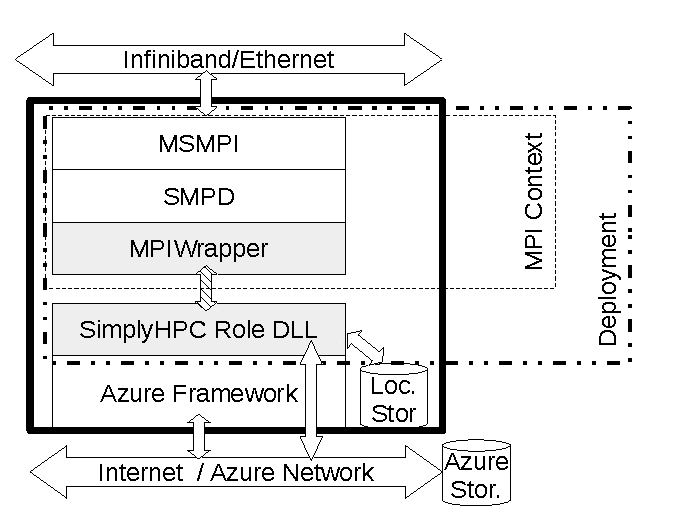
\includegraphics[width=.5\linewidth]{azureWorkerRole.pdf}
	\caption{Schematic view of a single compute node on Azure}

	\label{fig:schemaRole}
\end{figure}

It is important to note that this node architecture applies to all nodes in a cloud cluster, and is automatically configured using the aforementioned deployment package. The node with the lowest node id (usually 0) is subsequently called \textit{head node}.


\subsection{Cluster architecture}

Fig.~\ref{fig:schemaService} visualizes all relevant components of a deployed HPC cluster that has been set up using the SimplyHPC framework. 
A \textit{cloud service} (dashed rectangle in figure) is a bundle of multiple nodes using the same deployment template. Using the logical entity of a cloud service, nodes can be easily configured in terms of their number, size and the virtual network they belong to. 

When using A8/A9 nodes for scientific computing, the internode network (depicted as the upper arrow in Fig.~\ref{fig:schemaService}) is realized with Infiniband. In this mode all internode storage and MPI requests are transparently redirected to this very low latency, high bandwidth interconnect. Such configuration is crucial for performance with most parallel software.

The availability of fast internode connections strongly influences the choice of storage for different tasks. In total, our set up uses four storage types:
\begin{itemize}

	\item \textit{Azure Table Storage} is a schemaless database accessible by HTTP/REST. SimplyHPC takes advantage of table storage to store configuration information, node synchronization data and job meta data. Table storage is read and written by all nodes (Arrow 'A' in Fig.~\ref{fig:schemaService}).
	
	\item \textit{Azure Blob Storage} is a storage service used to store large data blocks and is accessible by HTTP/REST. Job data such as geometry, matrices, etc. are uploaded from a client to the Azure Blob Storage, and are then copied to the much faster local storage by the head node (Arrow 'B' in Figure \ref{fig:schemaService}). Job results are also uploaded back to this storage and thus made available via internet.	
	
	\item \textit{Azure File Storage} provides a storage which is mountable as a network drive in Windows, and is here used to make software packages available to the worker roles. Large software suites such as ANSYS cannot be included into deployment packages due to its size and can therefore not be directly installed on the PaaS worker roles. Here we used a prepared ANSYS installation on a shared network drive.
	
	\item \textit{Local Storage} is used during job execution for job data (Arrows 'C' in Fig.~\ref{fig:schemaService}). Local storage is realized using local SSD drives and can be shared between nodes using the SMBv3 Protocol and Infiniband. Local Storage is the fastest storage available currently on Microsoft Azure. It is important to note that local storage is not persistent, its data is lost after a node has been recreated, restored or updated. Also, local storage is not directly accessible outside the cloud service.

\end{itemize}


\begin{figure}[ht]
	\centering
	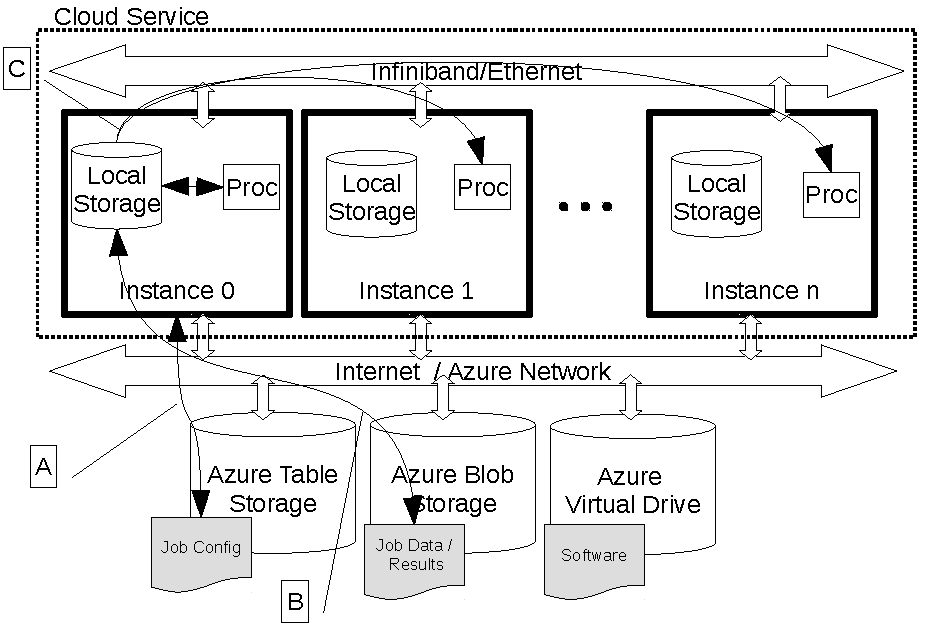
\includegraphics[width=.6\linewidth]{azureDeployment.pdf}

	\caption{Schematic view of a SimplyHPC Cluster on Azure}	
	\label{fig:schemaService}
\end{figure}

\subsection{Software architecture}

SimplyHPC has been written in .NET  /C\# and uses Azure mechanisms that automatize the process of setting up of the cluster described before. There are multiple levels at which the SimplyHPC interacts with Microsoft Azure.

It is linked to the Microsoft Azure SDK and uses parts of it to automatize the compilation of the deployment packages. On a runtime level, it interacts directly with the management interface of Microsoft Azure to create cloud services, upload deployment packages, monitor machine status etc.


We expose two different front ends to the user, namely PowerShell command-lets and a high-level API with a facade that hides all the complexity of orchestrating the cloud.  PowerShell is a object-oriented command line environment used to script and automatize common tasks.

PowerShell command-lets are building blocks that allow administrators to prepare custom scripts. The PowerShell interface provides a number of useful command-lets needed to deploy a scientific application in the cloud, execute it, download the results back to the user and destroy the cluster ( see Tab~\ref{tab:CommandletsOfSimplyHPC}). 

\begin{table}
	\centering		
		\begin{tabular}{|l|l|}
		\hline
      \textbf{Commandlet} & \textbf{Description} \\ \hline
      NewAzureService & Create a new cloud service and the cluster \\ \hline
			NewAzureJob & Create and execute a new job \\ \hline
			NewAzureParameters & Create a set of parameters required by other command-lets    \\ \hline
			GetJobStatus & Get the status of a given job    \\ \hline
			GetJobResults & Get the results of a given job  \\ \hline
			GetAvailableRoleSizes & Get Available VMs with their roles and sizes \\ \hline
			RemoveAzureJobs & Remove Azure Jobs such as unfinished jobs \\ \hline
			RemoveAzureService & Remove the cloud service and destroy the cluster \\ \hline
    \end{tabular}
	\caption{Command-lets of SimplyHPC framework.}
	\label{tab:CommandletsOfSimplyHPC}
\end{table}

Figure \ref{simplyHPCArch} visualizes the high-level architecture of SimplyHPC.

\begin{figure}[h]
\centering
	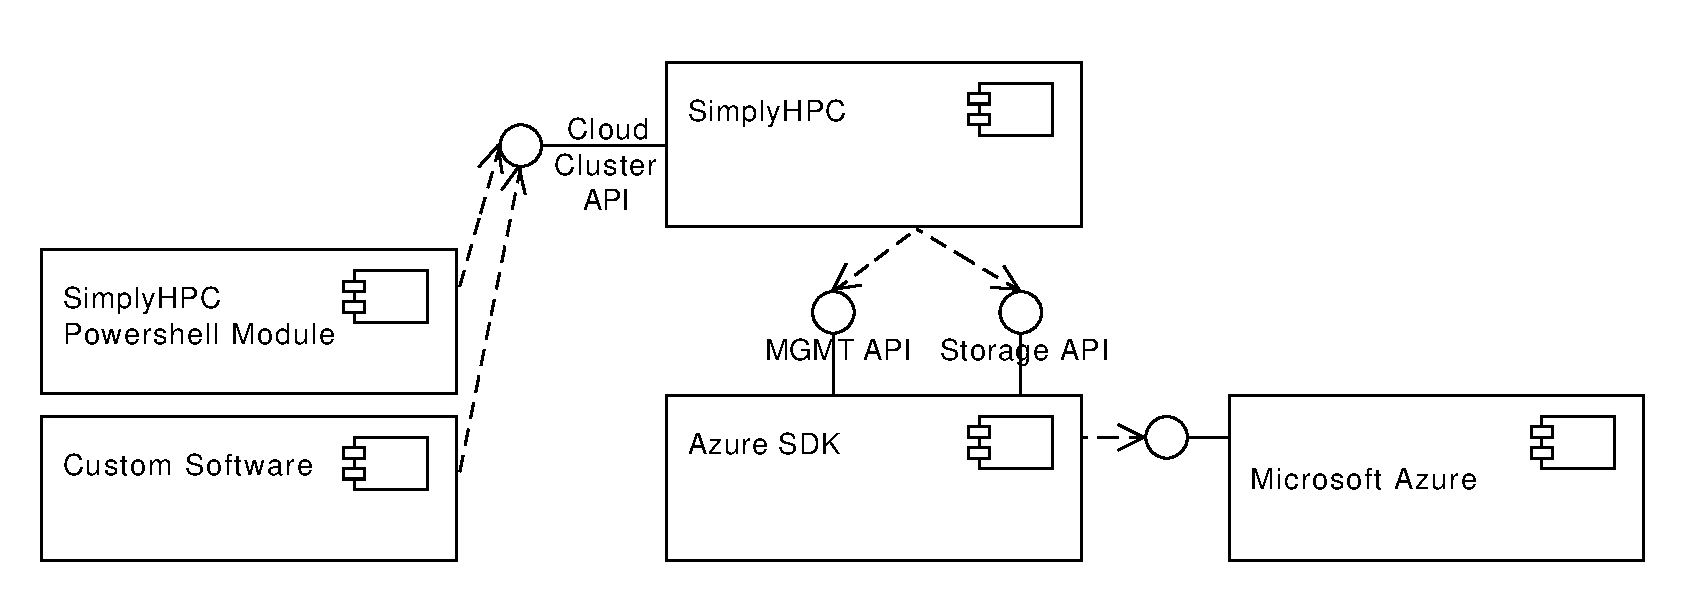
\includegraphics[width=.8\linewidth]{simplyHPCArch}
	\caption{Component Diagram of SimplyHPC}
	\label{fig:simplyHPCArch}
\end{figure}


\section{Results}
\label{sec:results}
In the following subchapters the measured performance of dynamic cloud clusters on Microsoft Azure are compared to a regular on-premises cluster using test cases relevant for CFD applications. Additionally, our SimplyHPC framework is compared to the standard HPC Pack approach in terms of set-up time of cloud clusters.

All tests were performed either on Microsoft Azure (Cloud Clusters) or on the HSR Cluster (On-Premises Clusters). HSR Cluster is a privately owned and maintained system at Microsoft Innovation Center at the University of Applied Sciences at Rapperswil (HSR), Switzerland. It is composed of $32$ nodes with 48GB RAM and two Intel Xeon E5645 6 cores each, the nodes are connected with 40Gbit Infiniband Network. On each node, Windows Server $2012$ R2 with HPC Pack 2012 R2 is installed.
On Microsoft Azure different node types were used: A8 (8 core Intel Xeon E5-2670, Infiniband interconnect) as well as A4 (shared CPU/GigE interconnect). For more detailed information about Microsoft Azure node types see table \ref{tab:azureVMs} resp. \cite{azure}.

\subsection{Set-up time}
The deployment time of a cloud cluster is crucial when using dynamically allocated systems, as they are newly set up for single jobs or a small series of jobs and taken down afterwards. These measurements obviously do not apply to on-premises clusters, as they are static.

Here we compared the time needed for setting up a cloud cluster consisting of A4 nodes with SimplyHPC and Microsoft HPC Pack. This time should be of the same order regardless the node size, because the deployment processes are similar. HPC Pack provides precise statistics on the deployment procedure separated into individual processes, namely creating a storage account, a virtual network, a cloud service, a domain controller as well as deployment and configuration time for the head node and compute nodes. Since in SimplyHPC most of these processes are omitted, only the time to deploy the head node and compute nodes was measured, e.g. the time needed to run \textit{NewAzureService} and \textit{NewAzureJob} scripts. Since HPC Pack neither provides automatic job submission nor does it retrieve the result we have not taken these processes into account in our measurements. 


\begin{figure}[h]
\centering
	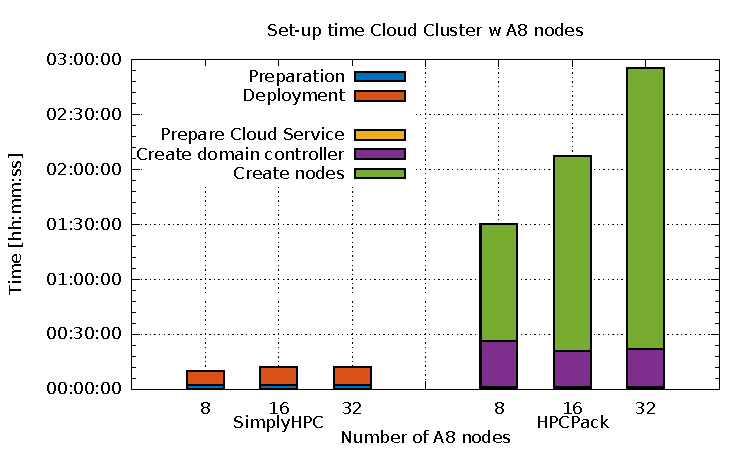
\includegraphics[width=.6\linewidth]{gplt-creation-simplyvshpc}
	\caption{Deployment time of cluster composed of different number of A4 nodes with Microsoft HPC pack (right) and SimplyHPC framework (left). Time is provided in hh:mm:ss format.}
	\label{fig:deployTime}
\end{figure}

Fig. \ref{fig:deployTime} shows the HPC Pack needs usually more than an hour to deploy a cloud cluster while SimplyHPC needs about ten minutes in average. The long deployment time of HPC Pack is due to the fact that HPC Pack deploys a fully functional cluster with a job scheduler, domain controller and SQL database. Although such a solution is desirable for business--oriented usage scenarios, there are many scenarios where applications need only an IaaS infrastructure and access to the MPI stack. In such a case the cluster can be deployed and destroyed much faster. Also, instead of deploying IaaS VMs sequentially like it is the case for HPC Pack, we just submit the deployment template to the cloud fabric with the request to set up a whole cloud service, consisting of multiple worker roles, simultaneously. This way the deployment time could be kept constant regardless of the cluster size.

\subsection{Sparse Matrix Solver Performance}
The objective of the second experiment was to compare the performance of a cloud cluster on Microsoft Azure with a traditional on-premises cluster using the example of distributed parallel sparse matrix solvers, as they are often used in CFD applications. The performance of these solvers depends on a multitude of factors such as CPU speed, memory bandwidth but also network speed and latency. Here we used 2 different solvers: The HPCG (High Performance Conjugate Gradients) Benchmark (see \cite{hpcg} for a detailed description) for standardized comparability and a PETSC (\cite{petsc}) solver with 2 different real world problems. PETSC is a widely used framework for scientific applications that includes parallel solver codes.
Both solvers were parallelized using Microsoft MPI (no OpenMP / threading).

On Microsoft Azure, the HPCG results scale nearly linearly with the number of cores, with a maximum speed-up of approx. $36$ with $64$ cores (compared to $1$ core) for A8 nodes. With A4 nodes, the scaling is not as desirable, probably also due to the lacking low-latency Infiniband interconnect. The dynamic cloud cluster easily outperforms the on-premises cluster. See fig. \ref{fig:hpcg} for more details.

PETSc was run with two different matrices: \textit{ruep} and \textit{nord}. The first one comes from a thermal transient heat conduction simulation of an electrical cabinet on a large unstructured mesh composed of 2.3 millions cells and the second matrix was generated from a thermal transient heat conduction simulation on a 3-dimensional Cartesian mesh of moderate size. Due to different mesh types, the second matrix converges much quicker than the first one.  \textcolor[rgb]{1,0,0}{IMPORTANT: SUPPLY MATRIX SIZES here!}

In figure \ref{fig:ruep} and \ref{fig:nord} the measurements for the PETSc trials are shown. On the cloud cluster using the A8 nodes scaling is close to ideal for the larger \textit{ruep} matrix, while the efficiency for large scaling decreases for the smaller \textit{nord} matrix. Using A4 nodes, scaling and performance are suboptimal - most likely due to the shared infrastructure and missing Infiniband interconnect.  The performance of the on-premises cluster is suboptimal in both cases. This is in part due to process starvation - the memory bandwidth is insufficient for this configuration and code. The same process layout was used on both systems (Azure/On-premises) and seems to be very unfavorable in the on-premises case.

Based on these results, especially the huge difference in performance between A8 and A4 nodes, only cloud clusters with A8 nodes are taken into account for subsequent tests with ANSYS CFX on Microsoft Azure.





\begin{figure}[h]
\centering
\begin{subfigure}{.33\textwidth}
	\centering
	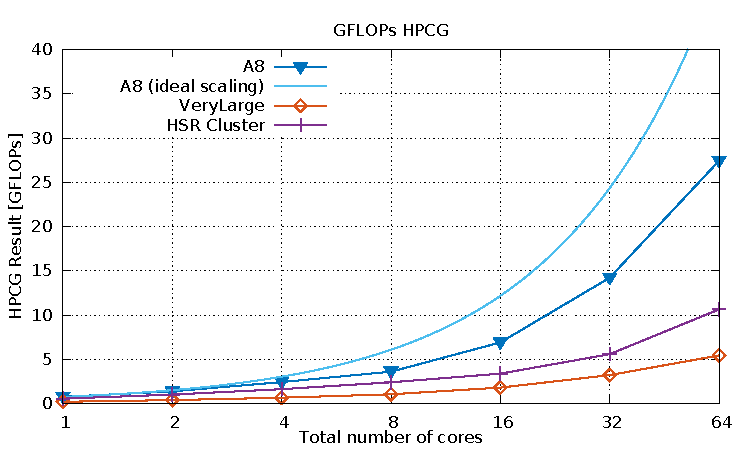
\includegraphics[width=\linewidth]{gplt-gflops-hpcg}
	\caption{HPCG}

	\label{fig:hpcg}
\end{subfigure}
\begin{subfigure}{.33\textwidth}
  \centering
	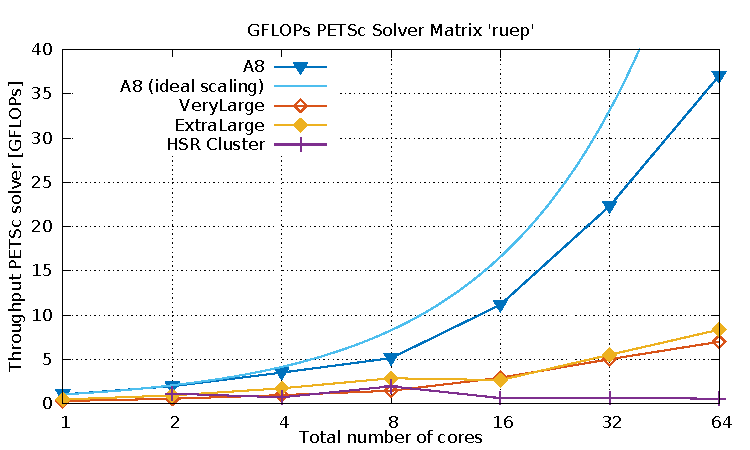
\includegraphics[width=\linewidth]{gplt-gflops-ruep}  

	\caption{PETSc with Matrix 'ruep'}
  \label{fig:ruep}
\end{subfigure}%
\begin{subfigure}{.33\textwidth}
  \centering
  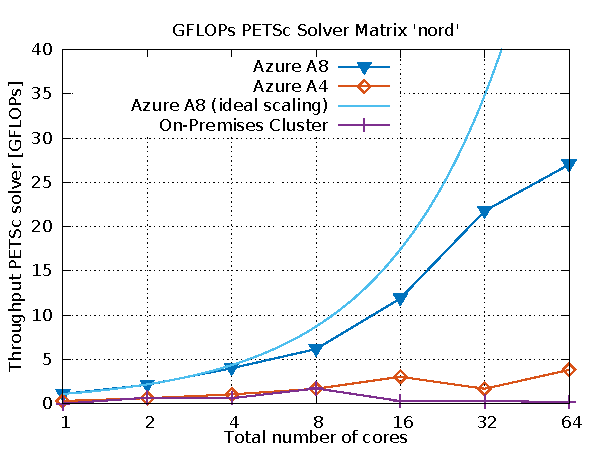
\includegraphics[width=\linewidth]{gplt-gflops-nord}
	\caption{PETSc with Matrix 'nord'}
  \label{fig:nord}
\end{subfigure}

\caption{Performance in GFlops of HPCG resp. PETSc solvers on cloud clusters with different node sizes on Microsoft Azure and on a on-premises cluster (HSR cluster) }
\label{fig:test}
\end{figure}


 

\subsection{ANSYS CFX Performance Study}
We used ANSYS CFX as an example of a widely used tool for large physical simulations.
Two independent simulations were run: a heat transfer simulation in a heat exchange system (subsequently called the \textit{pipe} case) and a fluid flow simulation in a compressor used in turbines (subsequently called the \textit{compressor} case).

The heat exchange system is composed of a buried pipe which is heated by an external source with a temperature of  $10 ^\circ C$. Water flows inside the pipe with a speed of $0.1m/s$. Such pipe heating systems are used to optimize energy costs in buildings through the reuse of energy. In this use case, the heat transfer to the flowing water is simulated. A visualization of the problem geometry is available in Fig.~\ref{fig:pipe}. By taking advantage of symmetrical problem geometry, test cases in different sizes (\textit{pipe01-pipe08}) were constructed by varying the coarseness of the mesh in x-direction. Using these test cases, the measurement of weak scaling is possible (fixed problem size per processor).

In the compressor model, air enters to the compressor through a filtered intake that removes the contaminants at the speed of $2.83\ m/s$ at $9.85 ^\circ C$. It then enters a space with three rotors where the air is compressed. Geometries of both systems are presented in Fig.~\ref{fig:geometries}. 
The coarseness of the first mesh can be varied  in x-direction due to the symmetrical geometry (cases pipe01-pipe08), while the mesh of the compressor case is fixed and has approx 13 million cells (see Tab~\ref{tab:MeshSize}). In both cases we modeled the steady state flows with residual targets of $1e-06$ resp. $1e-08$ and maximal number of iterations of $200$ and $100$, respectively. 

\begin{table}
	\centering
		\begin{tabular} {|c|c|c|}
			\hline
			Name & No. of Elements & No. of nodes \\			
			pipe01 & 195'102 & 255'462 \\ \hline
			pipe02 & 432'919 & 512'212 \\ \hline
			pipe06 & 1'017'573 & 1'148'856 \\ \hline
			pipe04 & 2'037'710 & 2'213'036 \\ \hline
			pipe05 & 4'010'210 & 4'313'036 \\ \hline			
			pipe07 & 8'101'299 & 8'526'790 \\ \hline
			pipe08 & 15'522'778 & 16'157'192 \\ \hline
			compressor & 13'799'389  & 11'025'383 \\ \hline
		\end{tabular}
	\caption{The mesh sizes of the test cases}
	\label{tab:MeshSize}
\end{table}

\begin{figure}
\centering
\begin{subfigure}{.4\textwidth}
	\centering
	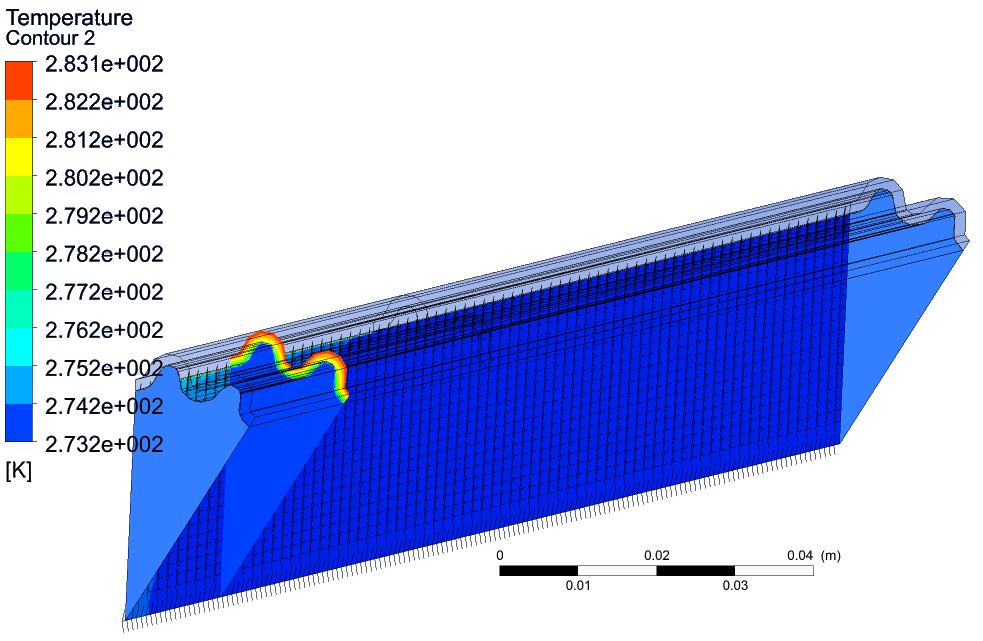
\includegraphics[width=\linewidth]{pipe_nobg}	
	\caption{Heat exchange system (\textit{pipe01-08})}
 	\label{fig:pipe}
\end{subfigure}
\begin{subfigure}{.5\textwidth}
	\centering
	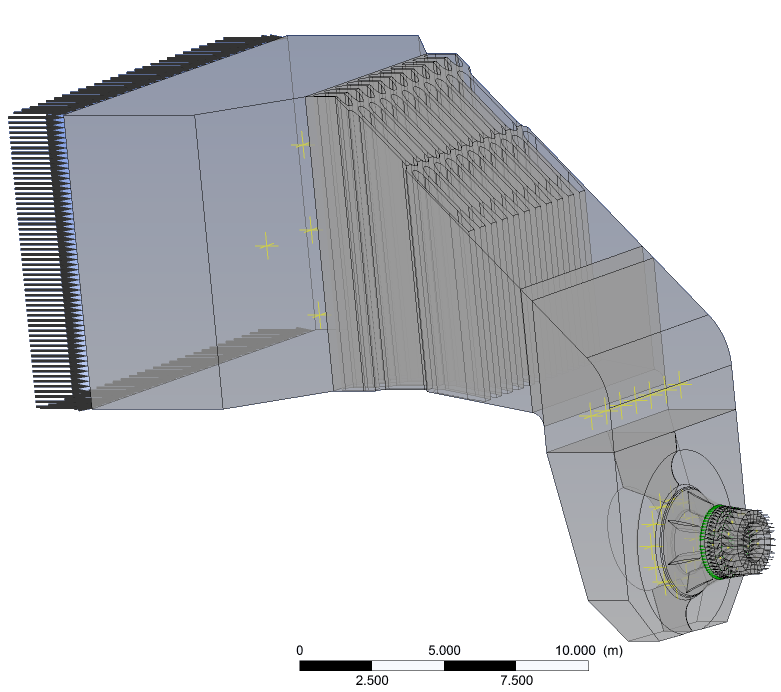
\includegraphics[width=.7\linewidth]{compressor_nobg}
	\caption{Compressor}
	\label{fig:compressor}
\end{subfigure}

\caption{Geometries of the used simulations.}
\label{fig:geometries}
\end{figure}


%%%%%%%%%%%%%%%%%%%%%%%%%%%%%%%%%%%%%%%%%%%%%%%%%%%
\subsubsection{Strong scaling of the heat exchange simulation}
\begin{figure}

	\begin{subfigure}{\textwidth}
		\centering
		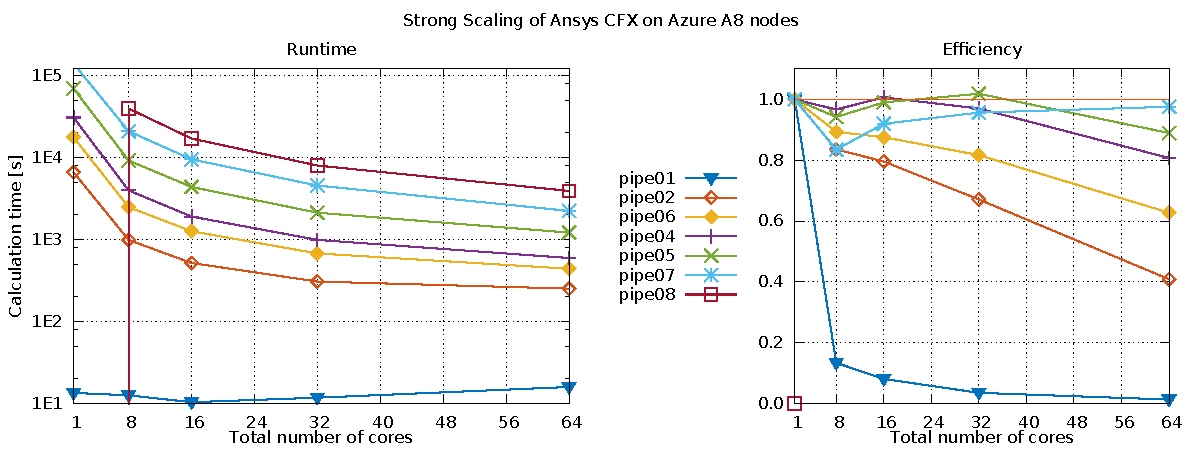
\includegraphics[width=.7\linewidth]{gplt-a8-strong-pipe}	
		\caption{Cloud Cluster}
		\label{fig:strongA8}
	\end{subfigure}

		\begin{subfigure}{\textwidth}
			\centering
			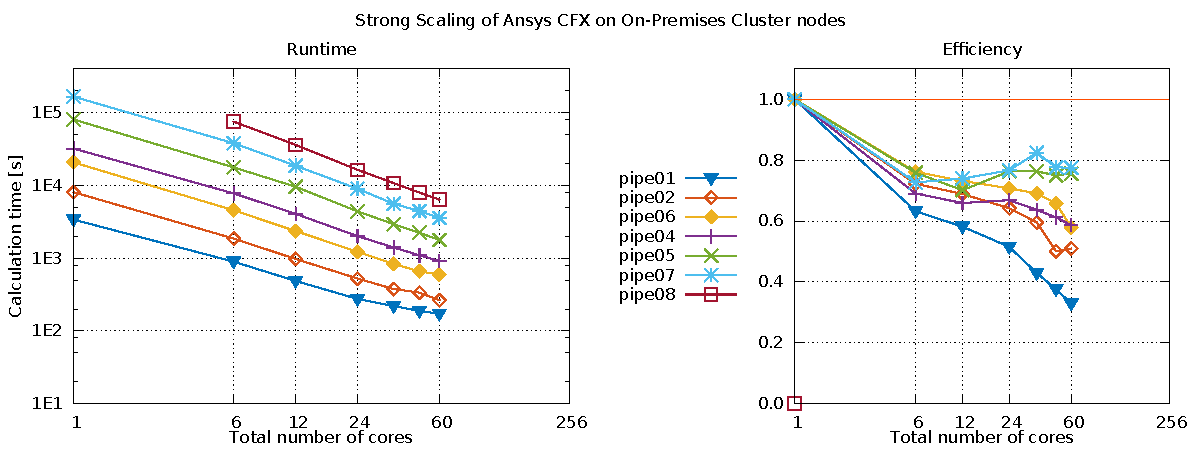
\includegraphics[width=.7\linewidth]{gplt-hsr-strong-pipe}
			\caption{On-Premises Cluster}
			\label{fig:strongHSR}
		\end{subfigure}
	\caption{Runtime and strong scaling efficiency of ANSYS CFX for pipe01-pipe08}
\end{figure}

For the strong scaling tests, the pipe01-pipe08 problems were solved on different cluster configurations. Note that the largest problem, pipe08, produced a memory overflow in a one core configuration and therefore the pipe08 strong scaling efficiency could not be computed. For the other cases, the strong scaling efficiency has been calculated accroding to Eq. \ref{eq:efficencyStrong}. For the second largest problem, pipe07, the sequential runtime is extrapolated, as 180 of 200 iterations could be calculated before the memory overflow and the increase of calculation time per iteration is a approximately constant fraction.



\begin{equation}
\label{eq:efficencyStrong}
E_s(N,K) = S(N,K) / K 
\end{equation}
where $S(N,K)$ is the speedup achieved on $K$ cores for the full problem size ($N$). The speedup is calculated according to Eq. \ref{eq:speedup}.

\begin{equation}
\label{eq:speedup}
S(N,K) = \frac{T_{seq}(N,1)}{T_{par}(N,K)}
\end{equation}
where $T_{seq}(N,1)$ is the runtime of the full problem (size $N$) using a sequential implementation of the solver on 1 core and $T_{par}(N,K)$ the runtime of a parallel implementation on $K$ cores, respectively (see \cite{kaminsky15} for more details).


Both systems showed good scaling for ANSYS	 CFX (see Fig. \ref{fig:strongA8} resp. \ref{fig:strongHSR}). The runtime is comparable, altough the strong scaling efficiency on the cloud cluster is much better - this might be due to memory bandwith limitations on the on-premises cluster (scaling from 1 to 6 greatly decreased efficiency).  Large cloud clusters (e.g. 128 cores in 32 nodes) need large problems to fully utilize their capabilities, the strong scaling efficiency for small problems rapidly decays. Even for larger problems the efficiency is suboptimal with 256 cores - in part due to communication overhead. 
A test with 64 with a total of 512 cores resulted in a MPI Broadcast timeout which might be due to the inefficient use of MPI collective operations or suboptimal broadcast algorithms (also reflected in the measured communication overhead). A hybrid approach (multithreading together with MPI) and/or MPI tuning could circumvent such problems.

%%%%%%%%%%%%%%%%%%%%%%%%%%%%%%%%%%%%%%%%%%%%%%%%%%%
 
\subsubsection{Weak scaling of the heat exchange simulation}


\begin{figure}

	\begin{subfigure}{\linewidth}
		\centering
		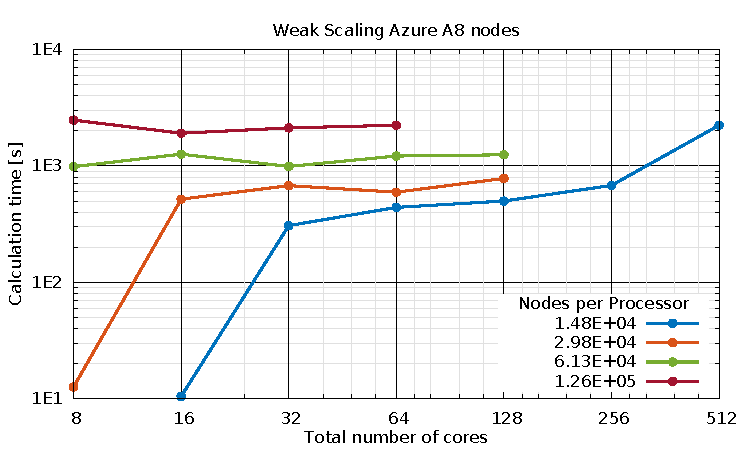
\includegraphics[width=.7\linewidth]{gplt-a8-weak-pipe}	
		\caption{Cloud Cluster}
		\label{fig:weakA8}
	\end{subfigure}

	\begin{subfigure}{\linewidth}
		\centering
		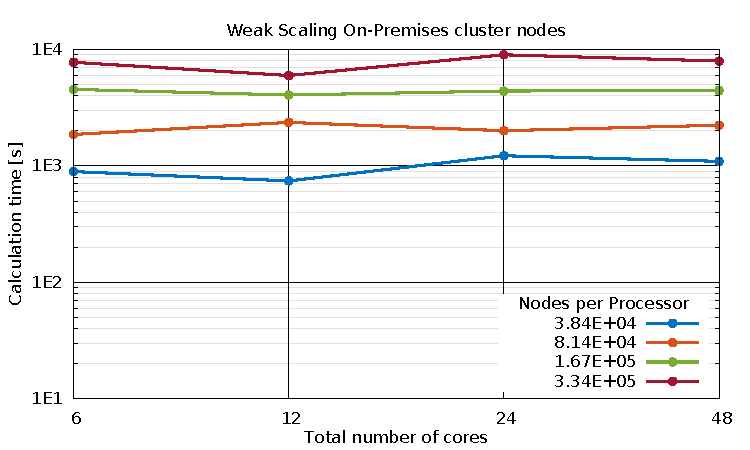
\includegraphics[width=.7\linewidth]{gplt-hsr-weak-pipe}
		\caption{On-Premises Cluster}
		\label{fig:weakHSR}
	\end{subfigure}
	
	\caption{Runtime and weak scaling efficiency of ANSYS CFX}

\end{figure}



In order to measure weak scaling and weak scaling efficiency the problem size per processor core is kept constant while increasing the number of processor cores. The weak scaling efficiency is calculated accoring to Eq. \ref{eq:efficiencyweak}.



\begin{equation}
	\label{eq:efficiencyweak}
	E_w(N,K) = S_u(N,K) / K
\end{equation}
where $S_u(N,K)$ is the size-up calculated according to Eq. \ref{eq:sizeup}, and $K$ is the number of cores.

\begin{equation}
\label{eq:sizeup}
S_u(N,K) = \frac{N(K)}{N(1)} \times \frac{T_{seq}(N(1),1)}{T_{par}(N(K),K).}
\end{equation}
where $N(K)$ resp. $N(1)$ is the problem size which is dependent on the number of cores $K$. This is due to the fact that the problem size is kept constant per core.
 Similarly to Eq.~\ref{eq:speedup}, $T_{seq}(.)$ denotes the running time of a sequential implementation on a single core. 

For more information about speedup/sizeup and strong/weak scaling efficiency, see \cite{kaminsky15}.



In Figure \ref{fig:weakA8} resp. \ref{fig:weakHSR} the weak scaling measured on cloud clusters and the on-premises cluster is visualized. For ideal weak scaling a horizontal curve is observed, as the increase of problem data is proportional to the increase of cores. Here it is also evident that for large problems both clusters scale well. 




\subsubsection{Performance compressor simulation}


\begin{figure}
	\centering
	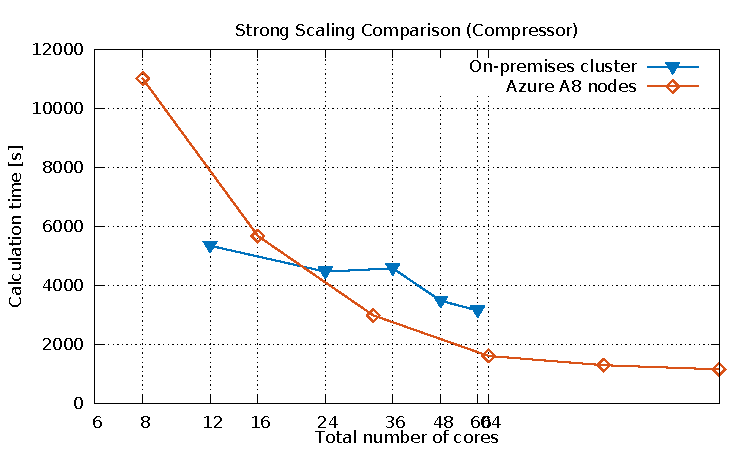
\includegraphics[width=0.5\linewidth]{gplt-compressor}
	\caption{Strong scaling for the compressor test case. }
	\label{fig:stringCompressor}
\end{figure}

 
\section{Conclusion}
\label{sec:conclusions}

We presented SimplyHPC framework, a novel distributed framework for Microsoft Azure Cloud. The framework is composed of a light--weight API and a set of commandlets on top of that. The modules automate the complex deployment procedure that is necessary to run third-party applications from the local machine. Specially designed mechanism keeps track of running jobs in the cluster. A special service in the head node regularly checks the job status and uploads the results to the blob storage as soon as the job finished successfully. Since a table and blob storage are distributed and mirrored, a high-availability and persistence of the job data is also provided. In contrary to HPC Pack from Microsoft, all unnecessary system components and services have been omitted. As a result the time needed to deploy the cluster has been reduced from more than an hour to couple of minutes.  We have demonstrated that the framework supports the deployment of both commercial and the open--source application on the cluster provided they are MPI--based and have a command line interface. scientific Big Data applications from Computational Fluid Dynamics domain, where both input and output data are usually massive. We also show that for extreme scaling  fine-tunning the hardware configuration is still necessary.
\begin{figure}
	\centering
	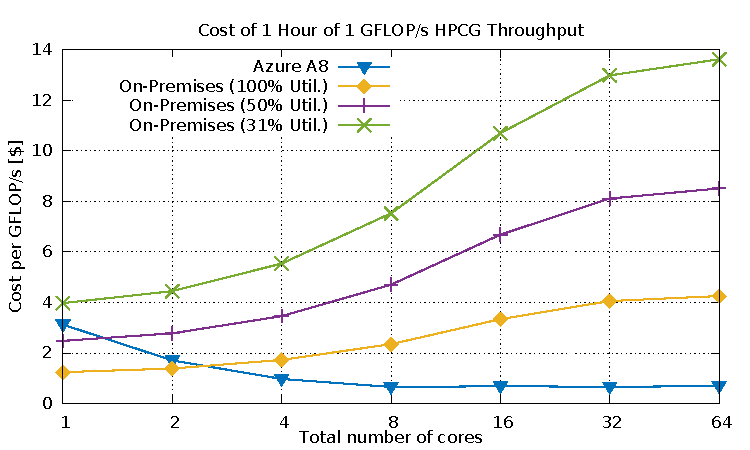
\includegraphics[width=.5\linewidth]{gplt-cost}
	\caption{Comparison of costs for Azure and a On-Premises Cluster}
	\label{fig:costs}
\end{figure}

We presented SimplyHPC framework, a novel distributed framework for Microsoft Azure Cloud. The framework is composed of light weight modules and a set of command-lets on top of that. The modules automate the complex deployment procedure that is necessary to run third-party applications from the local machine. In contrary to HPC Pack from Microsoft, all unnecessary system components and services have been omitted. As a result the time needed to deploy the cluster has been reduced from nearly an hour to couple of minutes.  This way scientific applications can access the cloud if the calculations are too time-consuming for a local machine or a private cluster. Specially designed mechanism keeps track of running jobs in the cluster. A special service in the head node regularly checks the job status and uploads the results to the blob storage as soon as the job finished successfully. Since a table and blob storage are distributed and mirrored, a high-availability and persistence of the job data is also provided. SimplyHPC software is available at GitHub at https://github.com/vbaros/SimplyHPC.

The paper clearly shows that scientists and engineers applications can access the cloud if the calculations are too time--consuming for a local machine or a private cluster and that they can benefit from competitive prices. Today, it is possible to deploy a 64--cores cluster for less than $\$30$ and this price is likely to be lower when the reader reads this paper. SimplyHPC software is available at GitHub at https://github.com/vbaros/SimplyHPC.


%\textcolor[rgb]{1,0,0}{mpantic: Additional suggestions for conclusion: Something about elasticity and cost efficiency, such as "Clearly, dynamic cloud clusters can compete with traditional on-premises clusters performance wise. Additionally, cloud clusters enable very cost efficient calculations as they are billed by the hour....etc etc}


%Further areas of work could include the following:

\section{Acknowledgments}
\label{sec:ackn}

The framework has been developed in Microsoft Innovation Center in Rapperswil, Switzerland. The scalability tests have been performed in Microsoft Azure as a part of Microsoft Research Grant No. Azdem187T64934Y. We would like also express our gratitude to Adrian Rohner, Roman Fuchs, Rita Rueppel and Vladimir Baros from University of Applied Sciences in Rapperswil for support and fruitful discussions.

\section{Literature}
\label{sec:literature}

\bibliography{fcgs}
\bibliographystyle{plain}

\end{document}


